\documentclass{standalone}
\usepackage{tikz}
\usetikzlibrary{patterns, positioning}
\usepackage[sfdefault]{ClearSans} %% option 'sfdefault' activates Clear Sans as the default text font
\usepackage[T1]{fontenc}

\begin{document}
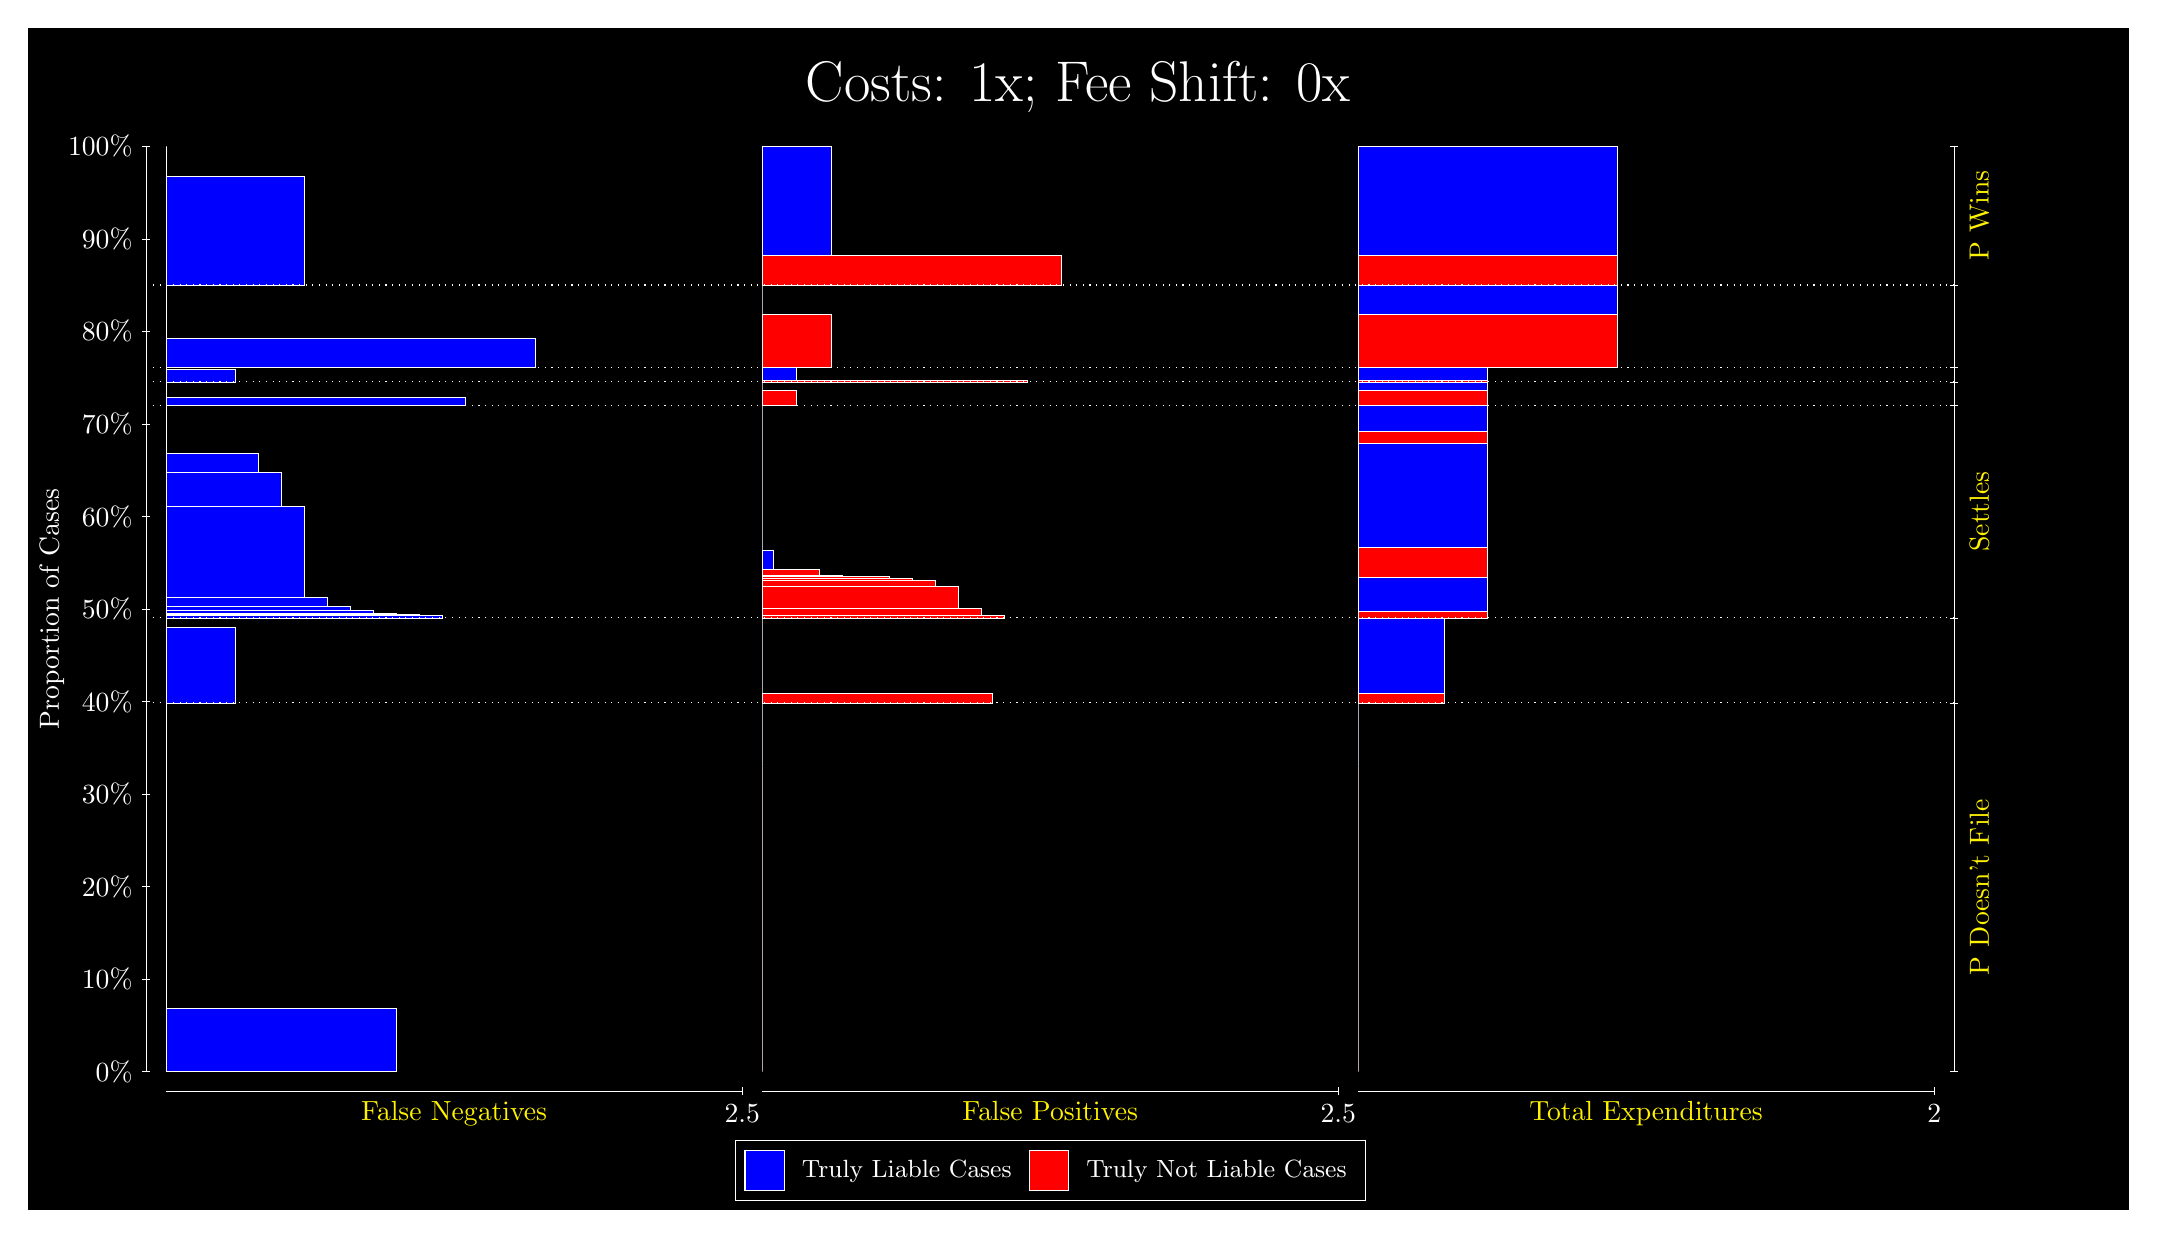
\begin{tikzpicture}
\draw[fill=black] (0,0) rectangle (26.667,15);
\draw[text=white] (0,13.5) rectangle (26.667,15) node[midway] {\huge Costs: 1x; Fee Shift: 0x};
\draw[white, very thin] (1.5,1.75) -- (1.5,13.5);
\node[rotate=90, text=white, anchor=center] at (0.3, 7.625) {Proportion of Cases};
\draw[white, very thin] (1.45,1.75) -- (1.55,1.75);
\node[text=white, anchor=east] at (1.45, 1.75) {0\%};
\draw[white, very thin] (1.45,2.925) -- (1.55,2.925);
\node[text=white, anchor=east] at (1.45, 2.925) {10\%};
\draw[white, very thin] (1.45,4.1) -- (1.55,4.1);
\node[text=white, anchor=east] at (1.45, 4.1) {20\%};
\draw[white, very thin] (1.45,5.275) -- (1.55,5.275);
\node[text=white, anchor=east] at (1.45, 5.275) {30\%};
\draw[white, very thin] (1.45,6.45) -- (1.55,6.45);
\node[text=white, anchor=east] at (1.45, 6.45) {40\%};
\draw[white, very thin] (1.45,7.625) -- (1.55,7.625);
\node[text=white, anchor=east] at (1.45, 7.625) {50\%};
\draw[white, very thin] (1.45,8.8) -- (1.55,8.8);
\node[text=white, anchor=east] at (1.45, 8.8) {60\%};
\draw[white, very thin] (1.45,9.975) -- (1.55,9.975);
\node[text=white, anchor=east] at (1.45, 9.975) {70\%};
\draw[white, very thin] (1.45,11.15) -- (1.55,11.15);
\node[text=white, anchor=east] at (1.45, 11.15) {80\%};
\draw[white, very thin] (1.45,12.325) -- (1.55,12.325);
\node[text=white, anchor=east] at (1.45, 12.325) {90\%};
\draw[white, very thin] (1.45,13.5) -- (1.55,13.5);
\node[text=white, anchor=east] at (1.45, 13.5) {100\%};

\draw[white, very thin] (24.457,1.75) -- (24.457,13.5);
\draw[white, very thin] (24.407,1.75) -- (24.507,1.75);
\node[anchor=west] at (24.407, 1.75) {};
\draw[white, very thin] (24.407,6.4319) -- (24.507,6.4319);
\node[anchor=west] at (24.407, 6.4319) {};
\draw[white, very thin] (24.407,7.5125) -- (24.507,7.5125);
\node[anchor=west] at (24.407, 7.5125) {};
\draw[white, very thin] (24.407,10.213) -- (24.507,10.213);
\node[anchor=west] at (24.407, 10.213) {};
\draw[white, very thin] (24.407,10.509) -- (24.507,10.509);
\node[anchor=west] at (24.407, 10.509) {};
\draw[white, very thin] (24.407,10.689) -- (24.507,10.689);
\node[anchor=west] at (24.407, 10.689) {};
\draw[white, very thin] (24.407,11.739) -- (24.507,11.739);
\node[anchor=west] at (24.407, 11.739) {};
\draw[white, very thin] (24.407,13.5) -- (24.507,13.5);
\node[anchor=west] at (24.407, 13.5) {};

\draw[white, very thin, fill=blue] (1.75,1.75) rectangle (4.6775,2.5559);
\draw[white, very thin, fill=red] (1.75,2.5559) rectangle (1.75,6.4319);
\draw[white, very thin, fill=blue] (1.75,6.4319) rectangle (2.6283,7.3886);
\draw[white, very thin, fill=red] (1.75,7.3886) rectangle (1.75,7.5125);
\draw[white, very thin, fill=blue] (1.75,7.5125) rectangle (5.2631,7.5506);
\draw[white, very thin, fill=blue] (1.75,7.5506) rectangle (4.9703,7.555);
\draw[white, very thin, fill=blue] (1.75,7.555) rectangle (4.6775,7.5646);
\draw[white, very thin, fill=blue] (1.75,7.5646) rectangle (4.3848,7.6066);
\draw[white, very thin, fill=blue] (1.75,7.6066) rectangle (4.3848,7.6077);
\draw[white, very thin, fill=blue] (1.75,7.6077) rectangle (4.092,7.6531);
\draw[white, very thin, fill=blue] (1.75,7.6531) rectangle (3.7993,7.7713);
\draw[white, very thin, fill=blue] (1.75,7.7713) rectangle (3.5065,8.9263);
\draw[white, very thin, fill=blue] (1.75,8.9263) rectangle (3.2138,9.3577);
\draw[white, very thin, fill=blue] (1.75,9.3577) rectangle (2.921,9.5984);
\draw[white, very thin, fill=red] (1.75,9.5984) rectangle (1.75,10.213);
\draw[white, very thin, fill=blue] (1.75,10.213) rectangle (5.5558,10.318);
\draw[white, very thin, fill=red] (1.75,10.318) rectangle (1.75,10.509);
\draw[white, very thin, fill=blue] (1.75,10.509) rectangle (2.6283,10.673);
\draw[white, very thin, fill=red] (1.75,10.673) rectangle (1.75,10.689);
\draw[white, very thin, fill=blue] (1.75,10.689) rectangle (6.4341,11.063);
\draw[white, very thin, fill=red] (1.75,11.063) rectangle (1.75,11.739);
\draw[white, very thin, fill=blue] (1.75,11.739) rectangle (3.5065,13.122);
\draw[white, very thin, fill=red] (1.75,13.122) rectangle (1.75,13.5);
\draw[white, very thin, fill=red] (9.3189,1.75) rectangle (9.3189,5.626);
\draw[white, very thin, fill=blue] (9.3189,5.626) rectangle (9.3189,6.4319);
\draw[white, very thin, fill=red] (9.3189,6.4319) rectangle (12.246,6.5558);
\draw[white, very thin, fill=blue] (9.3189,6.5558) rectangle (9.3189,7.5125);
\draw[white, very thin, fill=red] (9.3189,7.5125) rectangle (12.393,7.5505);
\draw[white, very thin, fill=red] (9.3189,7.5505) rectangle (12.1,7.6346);
\draw[white, very thin, fill=red] (9.3189,7.6346) rectangle (11.807,7.917);
\draw[white, very thin, fill=red] (9.3189,7.917) rectangle (11.515,7.9826);
\draw[white, very thin, fill=red] (9.3189,7.9826) rectangle (11.222,8.0119);
\draw[white, very thin, fill=red] (9.3189,8.0119) rectangle (10.929,8.0128);
\draw[white, very thin, fill=red] (9.3189,8.0128) rectangle (10.929,8.0362);
\draw[white, very thin, fill=red] (9.3189,8.0362) rectangle (10.636,8.0437);
\draw[white, very thin, fill=red] (9.3189,8.0437) rectangle (10.344,8.0465);
\draw[white, very thin, fill=red] (9.3189,8.0465) rectangle (10.051,8.127);
\draw[white, very thin, fill=blue] (9.3189,8.127) rectangle (9.4652,8.3677);
\draw[white, very thin, fill=blue] (9.3189,8.3677) rectangle (9.3189,10.213);
\draw[white, very thin, fill=red] (9.3189,10.213) rectangle (9.758,10.404);
\draw[white, very thin, fill=blue] (9.3189,10.404) rectangle (9.3189,10.509);
\draw[white, very thin, fill=red] (9.3189,10.509) rectangle (12.686,10.525);
\draw[white, very thin, fill=blue] (9.3189,10.525) rectangle (9.758,10.689);
\draw[white, very thin, fill=red] (9.3189,10.689) rectangle (10.197,11.364);
\draw[white, very thin, fill=blue] (9.3189,11.364) rectangle (9.3189,11.739);
\draw[white, very thin, fill=red] (9.3189,11.739) rectangle (13.125,12.117);
\draw[white, very thin, fill=blue] (9.3189,12.117) rectangle (10.197,13.5);
\draw[white, very thin, fill=red] (16.888,1.75) rectangle (16.888,5.626);
\draw[white, very thin, fill=blue] (16.888,5.626) rectangle (16.888,6.4319);
\draw[white, very thin, fill=red] (16.888,6.4319) rectangle (17.986,6.5558);
\draw[white, very thin, fill=blue] (16.888,6.5558) rectangle (17.986,7.5125);
\draw[white, very thin, fill=red] (16.888,7.5125) rectangle (18.534,7.5967);
\draw[white, very thin, fill=blue] (16.888,7.5967) rectangle (18.534,8.0282);
\draw[white, very thin, fill=red] (16.888,8.0282) rectangle (18.534,8.4063);
\draw[white, very thin, fill=blue] (16.888,8.4063) rectangle (18.534,9.726);
\draw[white, very thin, fill=red] (16.888,9.726) rectangle (18.534,9.8781);
\draw[white, very thin, fill=blue] (16.888,9.8781) rectangle (18.534,10.213);
\draw[white, very thin, fill=red] (16.888,10.213) rectangle (18.534,10.404);
\draw[white, very thin, fill=blue] (16.888,10.404) rectangle (18.534,10.509);
\draw[white, very thin, fill=red] (16.888,10.509) rectangle (18.534,10.525);
\draw[white, very thin, fill=blue] (16.888,10.525) rectangle (18.534,10.689);
\draw[white, very thin, fill=red] (16.888,10.689) rectangle (20.181,11.364);
\draw[white, very thin, fill=blue] (16.888,11.364) rectangle (20.181,11.739);
\draw[white, very thin, fill=red] (16.888,11.739) rectangle (20.181,12.117);
\draw[white, very thin, fill=blue] (16.888,12.117) rectangle (20.181,13.5);
\draw[white, dotted] (1.5,6.4319) -- (24.457,6.4319);
\draw[white, dotted] (1.5,7.5125) -- (24.457,7.5125);
\draw[white, dotted] (1.5,10.213) -- (24.457,10.213);
\draw[white, dotted] (1.5,10.509) -- (24.457,10.509);
\draw[white, dotted] (1.5,10.689) -- (24.457,10.689);
\draw[white, dotted] (1.5,11.739) -- (24.457,11.739);
\draw[white, very thin] (1.75,1.5) -- (9.0689,1.5);
\node[text=yellow, anchor=north] at (5.4094, 1.5) {False Negatives};
\draw[white, very thin] (9.0689,1.45) -- (9.0689,1.55);
\node[text=white, anchor=north] at (9.0689, 1.45) {2.5};

\draw[white, very thin] (9.3189,1.5) -- (16.638,1.5);
\node[text=yellow, anchor=north] at (12.978, 1.5) {False Positives};
\draw[white, very thin] (16.638,1.45) -- (16.638,1.55);
\node[text=white, anchor=north] at (16.638, 1.45) {2.5};

\draw[white, very thin] (16.888,1.5) -- (24.207,1.5);
\node[text=yellow, anchor=north] at (20.547, 1.5) {Total Expenditures};
\draw[white, very thin] (24.207,1.45) -- (24.207,1.55);
\node[text=white, anchor=north] at (24.207, 1.45) {2};

\node[text=yellow, centered, rotate=90] at (24.777, 4.091) {P Doesn't File};

\node[text=yellow, centered, rotate=90] at (24.777, 8.8627) {Settles};



\node[text=yellow, centered, rotate=90] at (24.777, 12.619) {P Wins};

\draw (12.978300999999998,1.5) node[draw=none] (baseCoordinate) {};
\begin{scope}[align=center]
        \matrix[scale=0.5, draw=white, below=0.5cm of baseCoordinate, nodes={draw}, column sep=0.1cm]{
            \node[rectangle, draw, minimum width=0.5cm, minimum height=0.5cm, fill=blue] {}; &
            \node[draw=none, font=\small, text=white] (B) {Truly Liable Cases}; &
            \node[rectangle, draw, minimum width=0.5cm, minimum height=0.5cm, fill=red] {}; &
            \node[draw=none, font=\small, text=white] (B) {Truly Not Liable Cases}; \\
            };
\end{scope}

\end{tikzpicture}
\end{document}